\section{A shared model for prediction and semantics}
\label{sec:model}
We train the model to predict future observations and recognize categories
from a shared feature sequence. Figure~\ref{fig:targets} shows the training
tasks. Panel A predicts the next sensory slice from the observed prefix.
Panel B predicts the later outcome of an action. Panel C shows how membrane
accumulation and spikes process sequences, and which losses train the readouts.

\subsection{Inputs, features, and spikes}
Let $m$ identify a sensory stream and let
$x^m_{1:T}\in\R^{T\times D_m}$ contain $T$ feature slices with $D_m$ channels
per slice. A slice is the numerical feature vector presented at one sequence
position. The implementation uses $T=16$, with modality-dependent channel
counts. Learned input adapters and modality embeddings map these features
into a shared width-$d$ representation, where $d=96$.
The audio, image, text, and video adapters and their data sources are described
in Appendix~\ref{app:training}.

A spiking neuron retains a membrane variable between sequence positions.
Figure~\ref{fig:targets}C illustrates how incoming information accumulates
until the membrane crosses a threshold and emits a spike.
For sensory position $\tau$, its update is
\begin{equation}
 v_\tau=\beta u_{\tau-1}+I_\tau,\qquad
 s_\tau=\mathbf{1}[v_\tau>V_{\mathrm{th}}],\qquad
 u_\tau=v_\tau-V_{\mathrm{th}}s_\tau.
 \label{eq:lif}
\end{equation}
Here $I_\tau$ is the incoming current, $u_{\tau-1}$ is the previous post-reset
membrane value, $v_\tau$ is the value before reset, and $s_\tau$ is a binary
spike. The indicator $\mathbf{1}[\cdot]$ is one when its condition holds and
zero otherwise. The decay $\beta=0.85$ retains part of the preceding value, and the
threshold $V_{\mathrm{th}}=1$ determines whether a spike is emitted. The last
operation subtracts the threshold after a spike. During offline training,
surrogate derivatives supply a gradient through the threshold
\citep{neftci2019surrogate,yu2026beyondrate}.

The shared core has two Transformer blocks and four attention heads. Each
query attends to at most four causal positions, including itself. Spikes enter
the attention and feed-forward paths, while residual connections carry numerical
features. The learned representation is a numerical feature sequence.
This implementation evaluates finite input
sequences on conventional hardware; its sparse attention is specified in
Appendix~\ref{app:training}.

\begin{figure}[tbp]
\centering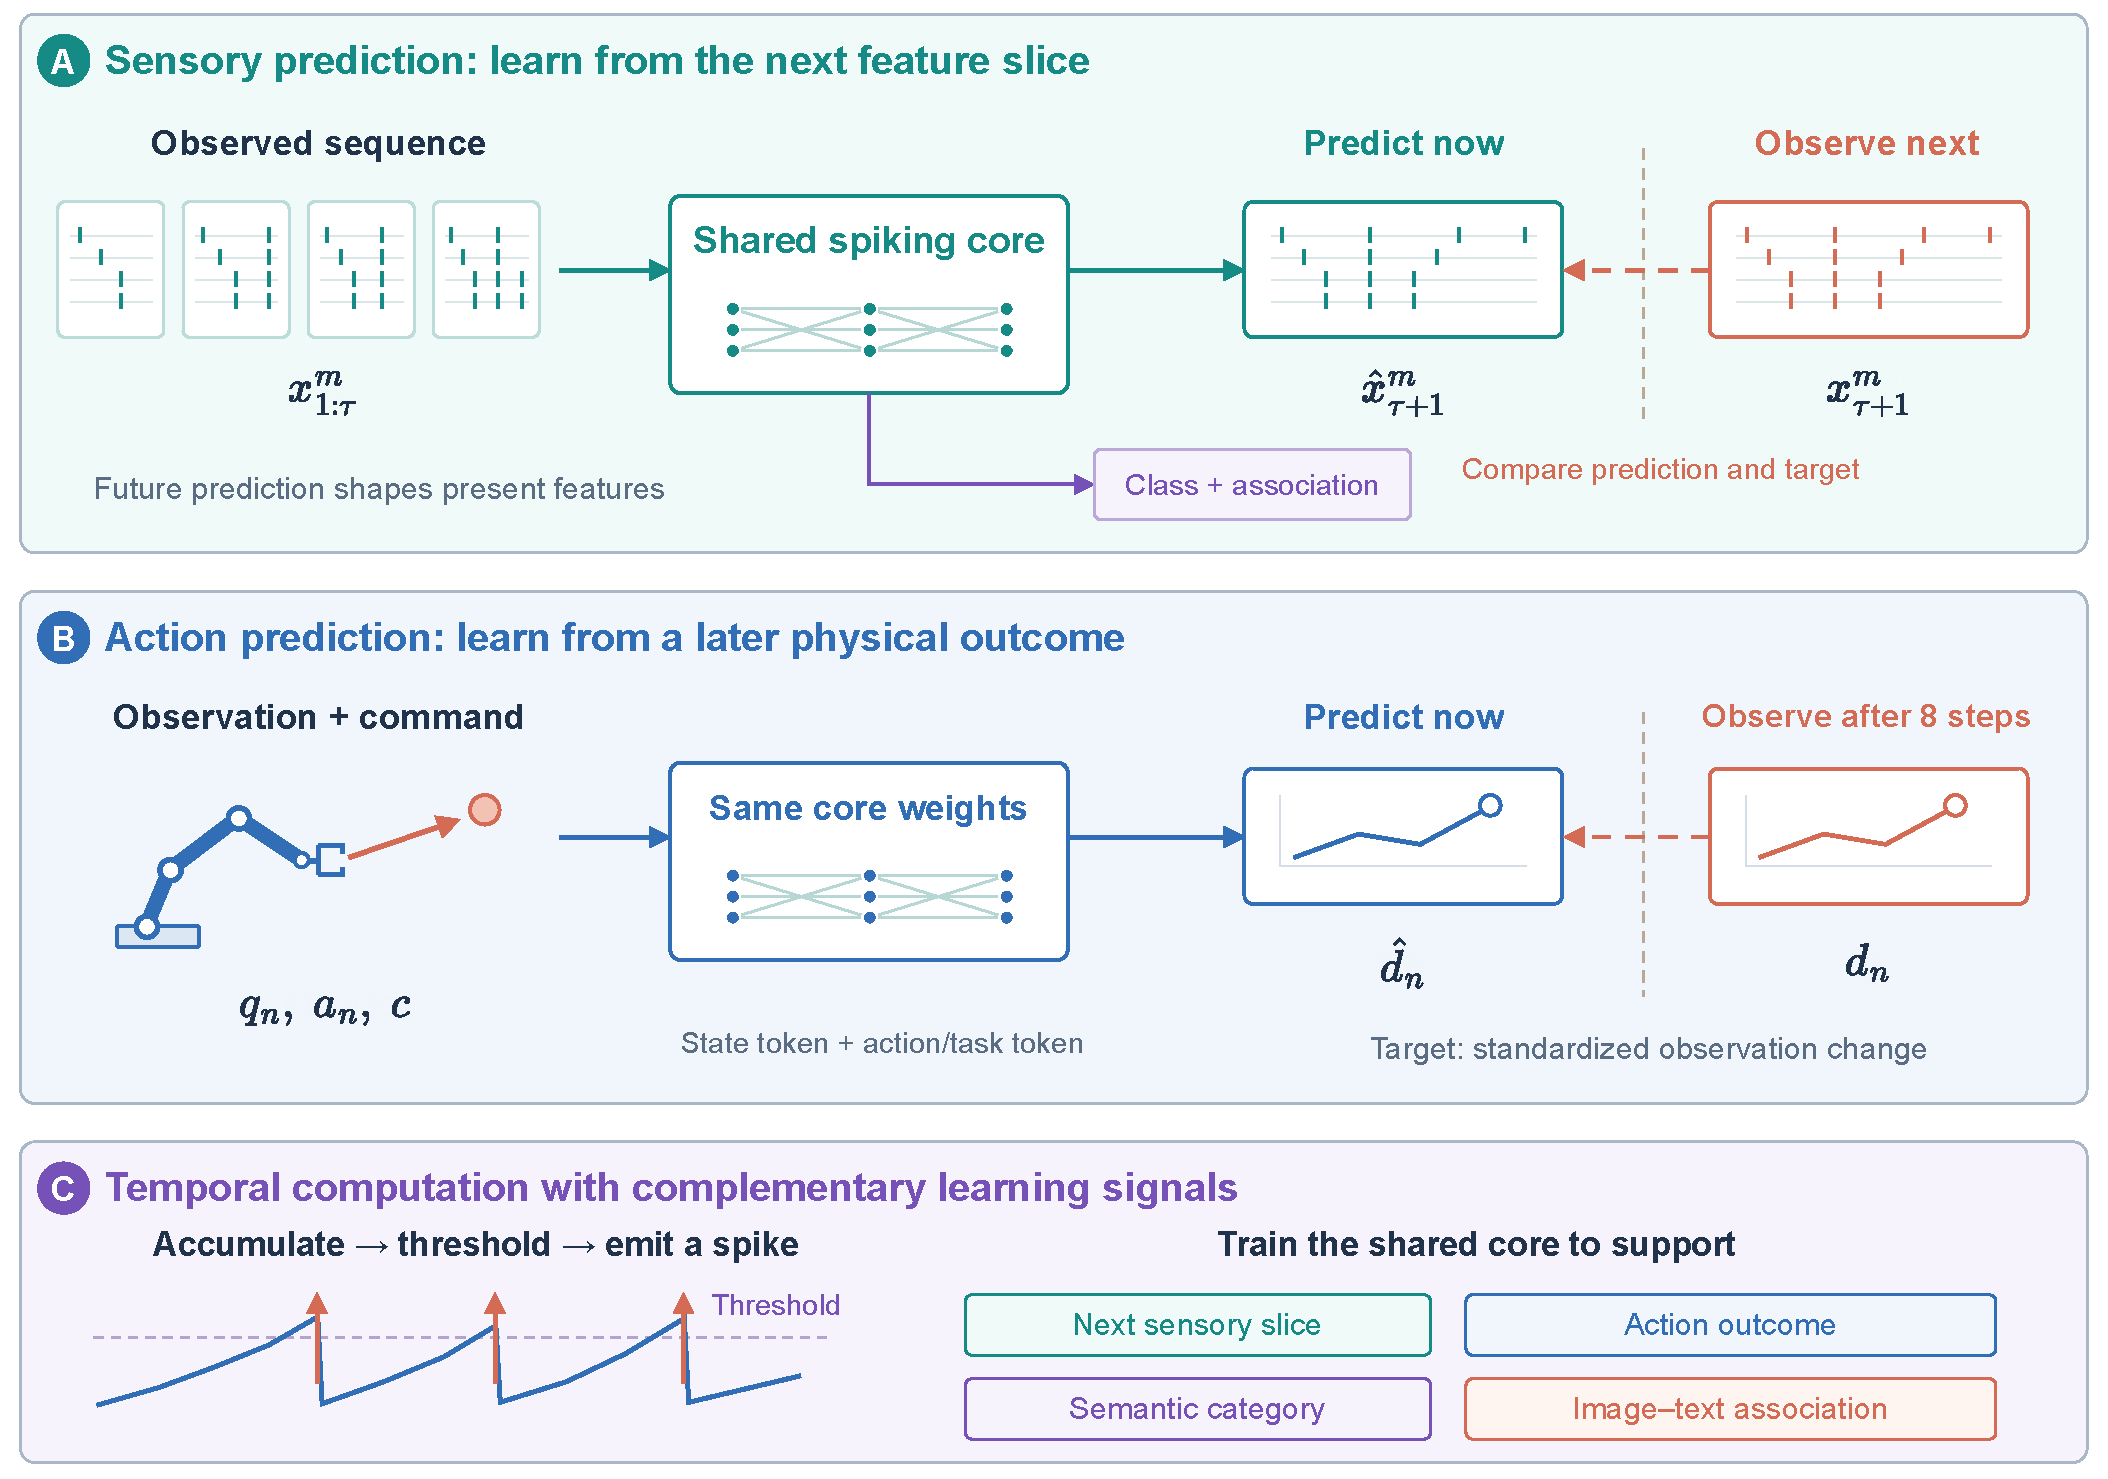
\includegraphics[width=\linewidth]{fig2_targets.pdf}
\caption{\textbf{Predict the next sensory slice and the later consequence of an action.}
\textbf{A}, the observed sensory prefix produces a next-slice prediction; the
next observation supplies its target. The same features also support class
recognition and association. \textbf{B}, current observation, command, and task
enter the same core to predict a standardized observation change, whose target
becomes available after eight environment steps. Dashed vertical lines separate
prediction time from target availability; coral arrows indicate target comparison.
\textbf{C}, membrane accumulation and thresholded spikes provide temporal
computation, while four objectives train complementary readouts of the shared
core. Sensory position $\tau$ and action decision $n$ use different clocks.
Feature patterns, trajectories, and membrane traces are schematic illustrations.}
\label{fig:targets}
\end{figure}

\subsection{Predicting the next sensory slice}
In Figure~\ref{fig:targets}A, the modality-specific output head uses positions
$1$ through $\tau$ to produce
$\hat x^m_{\tau+1}$, a prediction of the next feature slice. The hat marks a
prediction; $x^m_{\tau+1}$ without the hat is the observed target.
The prediction loss for stream $m$ is
\begin{equation}
 \ell_m=\frac{1}{(T-1)D_m\,p_m}
 \sum_{\tau=1}^{T-1}\|\hat x^m_{\tau+1}-x^m_{\tau+1}\|_2^2.
 \label{eq:next}
\end{equation}
The squared norm $\|\cdot\|_2^2$ sums squared errors across feature channels.
The outer sum then adds these errors over the available next-slice pairs.
Dividing by $(T-1)D_m$ averages over positions and channels. The positive
constant $p_m$ is the training-set error of the persistence baseline, which
predicts the next slice by copying the current one. This normalization puts
modalities with different numerical scales on comparable footing. The
sensory loss $\mathcal L_{\mathrm{next}}$ gives equal weight to audio, text,
image, and video groups. The audio group first averages its two sources,
SHD and SSC; Appendix~\ref{app:losses} gives the combined expression.

The core processes spikes, while the output adapters predict encoded feature
slices in each stream's feature space. The targets can therefore contain
non-binary values. Here, next-spike refers to causal prediction over these
event-oriented sensory sequences.

\subsection{Predicting action outcomes}
Figure~\ref{fig:targets}B uses a different horizon: the consequence of executing
a command. Use $n$ for a macro-decision and $t_n$ for its starting environment step.
An observation $q_n=q(t_n)\in\R^{D_q}$ has $D_q=39$ coordinates and contains
the simulator's numerical observation at the start of that decision. A command
$a_n\in[-1,1]^4$ and task identifier $c$ are supplied to the action branch.
Let $q_n^+=q(t_n+H)$ be the observed outcome after horizon $H=8$ environment
steps. The superscript $+$ marks this later observation. We predict how the
observation changes over the interval, using the standardized target
\begin{equation}
 d_n=(q_n^+-q_n-\mu_\Delta)\oslash\sigma_\Delta,
 \qquad
 \mathcal L_{\mathrm{act}}=\frac{1}{D_q}
 \|g_\theta(q_n,a_n,c)-d_n\|_2^2.
 \label{eq:action}
\end{equation}
Here $g_\theta$ is the action-conditioned predictor with trained parameters
$\theta$. The vectors $\mu_\Delta,\sigma_\Delta\in\R^{D_q}$ are the mean and
scale of training observation changes; $\oslash$ is coordinate-wise division.
Thus $d_n$ is a vector of observed changes, distinct from the scalar hidden
width $d$ introduced above.
The factor $1/D_q$ averages error over output coordinates. In the implementation
it is $1/39$, a dimensional normalization rather than a tuned coefficient.
The state and action/task adapters provide two tokens to the shared core;
the frozen linear endpoint head maps the final action feature to $D_q$ outputs.

\subsection{Learning predictions and semantic readouts together}
The four losses in Figure~\ref{fig:targets}C train prediction, recognition,
and association from the same core. The coupled semantic heads read its
features to predict category logits, the class scores before conversion to
probabilities.
Their cross-entropy loss is $\mathcal L_{\mathrm{sem}}$. A binding head maps
image and rendered-text features to normalized vectors, and a symmetric
contrastive loss $\mathcal L_{\mathrm{bind}}$ associates examples with the same
digit identity. Joint training minimizes
\begin{equation}
 \mathcal L_{\mathrm{joint}}=
 \mathcal L_{\mathrm{next}}+\mathcal L_{\mathrm{sem}}
 +\lambda_b\mathcal L_{\mathrm{bind}}+\lambda_a\mathcal L_{\mathrm{act}},
 \qquad \lambda_b=0.25,\quad\lambda_a=4.
 \label{eq:joint}
\end{equation}
The fixed coefficients $\lambda_b$ and $\lambda_a$ set the relative weights
of association and action prediction in the training loss.
Equation~\eqref{eq:joint} trains the core to preserve
information useful for both future prediction and present classification.
Appendix~\ref{app:losses} expands the classification and contrastive terms.

We evaluate two training stages separately.
The \emph{sequential checkpoint} begins with sensory pretraining and then trains
the action path for 800 updates while holding the core fixed. This is the
checkpoint used in the main deployment comparison. The \emph{joint checkpoint}
adds 200 shared-core updates with Equation~\eqref{eq:joint}. A separate study
compares these stages to measure the effect of joint learning. Once a checkpoint
is selected for deployment, all of its trained parameters are frozen.
